\documentclass[12pt,a4paper]{article}
\usepackage{geometry}
\usepackage{amsmath}
\usepackage{graphicx}
\usepackage[hidelinks]{hyperref}
\usepackage{float}
\usepackage{xcolor}

\geometry{margin=1in}

\title{\textbf{Feasibility Study: Automated Online Test Monitoring System}}
\author{}
\date{}

\begin{document}

\maketitle

\section*{Group Members}
\vspace{-5pt}
\begin{itemize}
    \item \textbf{Mohsen IranianGhareshiran} - 202382341
    \item \textbf{Galilea Le Moullec} - 202415993
    \item \textbf{Félicien Moquet} - 202415994
    \item \textbf{Kateryna Nazarenko} - [Student Number]
\end{itemize}

\noindent This document evaluates the feasibility of developing an \textbf{Automated Online Test Monitoring System} to ensure the \textbf{integrity and credibility} of online assessments while mitigating fraud and inefficiencies in remote test-taking environments.

\tableofcontents
\newpage

\section{Project Overview}

\subsection{Client Background}
With the increase in digital learning and remote assessments, it has become increasingly important to monitor online tests in a secure and automated manner. As well as individual educators conducting online exams, large-scale educational institutions and certification bodies administering high-stakes tests may utilize this system as clients.

In traditional online proctoring methods, human supervisors monitor test-takers via live video feeds. However, these methods present several challenges:
\begin{itemize}
    \item \textbf{High costs and logistical complexities} associated with hiring and managing manual proctors.
    \item \textbf{Difficulties in verifying candidate presence}, as test-takers may attempt to bypass monitoring systems.
    \item \textbf{Spoofing attacks}, where a test-taker may use \textbf{prerecorded videos, images, or digital manipulations} to create the illusion of presence.
    \item \textbf{It is challenging to coordinate global test sessions}, particularly when dealing with different time zones and availability restrictions.
\end{itemize}

To address these concerns, an automated exam proctoring system with artificial intelligence is proposed. This system does not require a human examiner to actively monitor candidates, unlike traditional proctoring solutions. As a result, it integrates seamlessly with existing examination platforms. Candidates are monitored in real time, and anti-spoofing checks are carried out without human intervention.

\subsection{Scope}

The Automated Online Test Monitoring System is designed to enhance the security and credibility of online assessments by providing real-time AI-powered monitoring and anti-spoofing mechanisms. This system serves as a feature that integrates with existing online exam platforms. It eliminates the need for manual proctoring during the exam.

\subsubsection{Included Features}

\begin{itemize}
    \item \textbf{Live Activity Detection} – Ensures test-takers remain present and engaged during exams using facial recognition and motion tracking.
    \item \textbf{Anti-Spoofing Measures} – Detects fraudulent attempts such as prerecorded videos, deepfake images, and screen replays.
    \item \textbf{Automated Reporting} – Generates detailed logs for administrators to review test sessions efficiently.
    \item \textbf{Scalability} – Supports large numbers of candidates without compromising system performance.
    \item \textbf{Time-Zone Adaptability} – Adjusts monitoring schedules to accommodate test-takers from different regions.
\end{itemize}

\subsubsection{Excluded Features}

\begin{itemize}
    \item \textbf{Cheating Detection Beyond Presence Monitoring} – The system does not track screen activity, keystrokes, or external devices.
    \item \textbf{Manual Proctoring} – There is no live human monitoring. Instead, AI automates the process.
    \item \textbf{Identity Verification Before the Exam} – The system focuses only on monitoring during the exam. It does not handle registration or ID verification.
\end{itemize}

It is important to note that our system does not completely replace human verification (registration, ID card verification for instance) as mentioned above.

\subsection{Project Objective}

With regard to this project, the primary objective is to develop an Automated Online Test Monitoring System that ensures the presence and active engagement of test-takers through artificial intelligence-driven activity detection and anti-spoofing techniques. In addition to eliminating the need for manual proctoring, this system also maintains test integrity by acting as an enhancement to existing online exam platforms.

The following are key objectives:

\begin{itemize}
    \item \textbf{Live Activity Detection} – Through the use of AI-based facial recognition and motion tracking, live activity detection ensures that the test-taker is physically present during the exam and engaged throughout.
    \item \textbf{Spoofing Mechanisms} – Detecting fraudulent behavior such as prerecorded videos, static images, or deepfake attempts.
    \item \textbf{Scalability and Compatibility} – Guarantee ease of use without disrupting student academic assessment (seamless integration with existing online examination platforms).
    \item \textbf{Time-Zone Flexibility} – Adjusting monitoring schedules to accommodate global exam schedules (allowing for flexibility for international test-takers)
    \item \textbf{Automated Reporting and Alerts} – Flagging suspicious activities and providing detailed logs for post-exam review by administrators.
\end{itemize}

Using artificial intelligence to power the system, educational institutions and certification bodies will be able to perform online assessments in a cost-effective, scalable, and reliable manner while reducing operational costs.

\section{Feasibility Analysis}


\subsection{Requirements}

\subsubsection{Functional Requirements}

\begin{table}[H]
    \centering
    \renewcommand{\arraystretch}{1.5}
    \begin{tabular}{| p{4cm} | p{6cm} | p{6cm} |}
        \hline
        \textbf{Requirement Type} & \textbf{Description} & \textbf{Exectution} \\
        \hline
        Real-time Monitoring & The system must detect the student's presence using facial recognition and gaze tracking. & The AI must analyze the webcam to ensure the student is in front of the screen. \\
        \hline
        Anti-Cheating Detection & Identify fraud attempts such as prerecorded videos or static images. & Detect deepfakes, printed photos, or suspicious movements. \\
        \hline
        Automated Reporting & Generate logs and alerts to flag suspicious behavior. & After the exam, the system generates a detailed report of detected anomalies. \\
        \hline
        Exam Platform Compatibility & Must integrate with platforms like Moodle or ExamSoft. & An API enables the exam platform to activate automated monitoring. \\
        \hline
        Time Zone Management & Adjust monitoring schedules to accommodate international candidates. & If a student is in Asia and another in Europe, the system adapts the schedule. \\
        \hline
    \end{tabular}
    \caption{Functional Requirements}
\end{table}


\subsubsection{Non-Functional Requirements}

\begin{table}[H]
    \centering
    \renewcommand{\arraystretch}{1.5}
    \begin{tabular}{| p{4cm} | p{6cm} | p{6cm} |}
        \hline
        \textbf{Requirement Type} & \textbf{Description} & \textbf{Execution} \\
        \hline
        Performance & The system must process real-time monitoring without excessive latency. & Video analysis should execute in less than 500 ms. \\
        \hline
        Data Security & No sensitive data should be stored permanently. & Store only the analysis results, not students' video footage. \\
        \hline
        Availability & The system must be accessible 24/7 for global exams. & Cloud-based hosting on AWS/GCP to ensure availability. \\
        \hline
        Scalability & Must support a large number of simultaneous users. & Ability to monitor 1,000 students in parallel. \\
        \hline
        Integration Ease & The system must integrate with LMS without major modifications. & A REST API enables communication with other platforms. \\
        \hline
        User-Friendly Interface & Simple and intuitive interface for students and administrators. & A dashboard that allows quick navigation and easy alert review. \\
        \hline
    \end{tabular}
    \caption{Non-Functional Requirements}
\end{table}

\subsection{Existing Systems}

Several online exam proctoring solutions are currently available (refer to References (A.3) below). The table below summarizes three widely used platforms, highlighting their advantages and disadvantages:

\begin{table}[H]
    \centering
    \renewcommand{\arraystretch}{1.3}
    \begin{tabular}{|l|p{6cm}|p{6cm}|}
        \hline
        \textbf{System} & \textbf{Advantages} & \textbf{Disadvantages} \\
        \hline
        \textbf{ProctorU} & 
        - Strong candidate authentication process. \newline
        - Supports high-stakes exams. 
        & 
        - Need of human proctors vigilance. \newline
        - Expensive due to human involvement. \newline
        - Privacy concerns related to live monitoring. \newline
        - Requires a stable internet connection. \\
        \hline
        \textbf{Proctorio} & - Fully AI-based, eliminating the need for human proctors. \newline
        - Seamless integration with LMS platforms. \newline
        - Cost-effective for large-scale exams. 
        & - High risk of false positives in fraud detection (moderate reliability). \newline
        - Concerns over data privacy \newline
        - Requires reliable technical infrastructure. \\
        \hline
        \textbf{Examity} & - Combines AI with human review for improved accuracy. \newline
        - Offers different levels of monitoring based on needs. \newline
        - Works with major learning platforms. 
        & - Expensive (particularly for fully monitored exams) \newline
        - Concerns over student data security \newline
        - Technical requirements may be an obstacle for some users \\
        \hline
    \end{tabular}
    \caption{Comparison of Existing Online Proctoring Systems}
\end{table}

\noindent Finally, these systems are on the whole costly and inaccessible to many institutions. What is more, they do not meet all requirements, especially when it comes to managing private data. These conclusions justify the proposal of a new solution.


\subsection{Technical Feasibility}

In order to ensure test integrity and eliminate the need for manual proctoring, the proposed Automated Online Test Monitoring System utilizes artificial intelligence. Based on its capacity to provide real-time monitoring, detect spoof attempts, and seamlessly integrate into existing exam platforms, the technical feasibility of the system is determined.

\begin{itemize}
    \item \textbf{Live Activity Detection}: The system utilizes AI-driven facial recognition, gaze tracking, and motion analysis to verify that the test-taker is physically present and actively engaged throughout the exam. In order to ensure that the candidate is attentive and focused on the exam screen, the system continuously tracks their facial features and head movements. In this manner, test-takers are prevented from leaving the exam session unnoticed or attempting to arrange for the test to be taken by someone else.

    \item \textbf{Anti-Spoofing Mechanisms}: There are various methods for spoofing traditional face recognition systems, including prerecorded videos, deep-fake-generated images, and static images. These threats can be addressed by incorporating advanced liveness detection techniques, including texture analysis, blinking detection, depth sensing, and real-time challenge-response interactions, to counter these threats. As a result of these techniques, it is possible to distinguish real human activity from deceptive attempts, thereby ensuring that the test-taker is physically present during the examination and interacting naturally with the environment.

    \item \textbf{Time Zone Awareness}: Online examinations cater to international candidates across different time zones; therefore, the system offers adaptive monitoring schedules based on the availability of test-takers across different time zones. In this manner, monitoring services remain effective regardless of geographical location, reducing disruptions for students. Moreover, automated scheduling and monitoring reports allow exam administrators to manage candidates from multiple time zones without requiring manual intervention.

    \item \textbf{Scalable Web-Based System}: An effective web-based system that can handle large numbers of concurrent users makes it suitable for both small institutions and large universities or certification bodies. Throughout the system, scalability is achieved by utilizing cloud-based deployment, load balancing, and a microservices architecture that allows the system to efficiently allocate resources to meet demand. In other words, as the number of test-takers increases, server resources are dynamically adjusted in order to maintain performance and reliability without causing system crashes or slowdowns.
\end{itemize}

\subsubsection{Technology Stack}

Using AI, web development frameworks, and cloud technologies, the system provides a secure, scalable, and efficient solution for online test monitoring.

\begin{itemize}
    \item \textbf{Machine Learning and AI}: A combination of TensorFlow, OpenCV, and ONNX is used for model training and real-time inference. These frameworks allow facial recognition, liveness detection, and motion tracking to ensure that the test-taker is present at the time of the test.

    \item \textbf{Facial Recognition}: The use of Convolutional Neural Networks (CNN-based models) to verify the identity of test-takers ensures that only authorized individuals are allowed to take the test.

    \item \textbf{Development of Web Applications}: The combination of Flask/Django (backend) with React/Angular (frontend) provides a seamless and user-friendly experience for administrators and test-takers.

    \item \textbf{Deployment on the Cloud}: The system is hosted on an AWS, Google Cloud, or Azure cloud, allowing for scalable infrastructure, high availability, and secure data storage.
\end{itemize}

As a result of integrating these technologies, the system provides an efficient, scalable, and secure solution for monitoring online tests, thereby eliminating manual proctoring and reducing costs.

\subsection{Organizational Feasibility}
\begin{itemize}
\item \textbf{Management Expertise}: Requires integration with existing learning management systems (LMS) or exam platforms.
\item \textbf{Technical Expertise}: A basic user-level understanding of web applications is required. Training will be provided to the user, and they will need to agree to install updates when available.

\item \textbf{Candidate Adaptability}: Test-takers may require clear instructions and onboarding to understand monitoring procedures.
\end{itemize}

\subsection{Financial Feasibility}

In this section, we examine the financial viability of this project by comparing current operating costs with projected project costs.

\subsubsection{Current Cost Analysis}
Currently, institutions spend approximately CAD\$230,000 annually on manual proctoring, including proctor salaries and administrative costs.

\subsubsection{Projected Cost Analysis}
With the implementation of an AI-based monitoring system, annual costs are estimated to be CAD\$80,000, including cloud infrastructure, AI retraining, and maintenance. The initial investment for development is CAD\$150,000.


\noindent Thus, the AI-based monitoring system will fully recover its investment in 1 year, making it a financially very viable and cost-effective solution for long-term online exam supervision.
For a detailed breakdown of these costs, refer to Appendix \ref{sec:cost_analysis}.

\section{Risks and Mitigation Strategies}

\subsection{Technical Risks}

\begin{itemize}
    \item \textbf{False Positives/Negatives}:  
    Artificial Intelligence models may occasionally misclassify test-taker behavior, resulting in unnecessary flaggings (false positives) or missed violations (false negatives), which can negatively impact the credibility of the system. To mitigate this, the AI models will undergo continuous refinement through extensive testing, retraining on a variety of datasets, and incorporating feedback from users to improve accuracy and reliability.

    \item \textbf{System Latency}:  
    Real-time facial recognition, liveness detection, and motion analysis require substantial computational power. The effectiveness of live monitoring may be compromised by delays in processing, resulting in lagging responses and potential disruptions. As a result, algorithm optimization techniques, such as model quantization and hardware acceleration, will be explored. However, due to limited computational resources, real-time efficiency cannot always be guaranteed.

    \item \textbf{Computational Resource Limitations}:  
    The performance of the system may be limited by hardware limitations, particularly when the AI models are run on a standard cloud-based or on-premise system. In spite of the ideal solution of scaling up resources, this may not always be possible as a result of budget constraints or infrastructure constraints. Consequently, all code and training processes will remain open, allowing full optimization of the system once the necessary computational requirements are met.

    \item \textbf{Data Privacy and Security}:  
    The system deals with sensitive biometric data, so privacy and security are important concerns. Thus, following the completion of the exam, only the final AI-generated results of the monitoring process will be saved, not recorded video footage. In this manner, the privacy of test-takers is maintained while ensuring the integrity of the examination records is maintained.
\end{itemize}


\subsection{Organizational Risks}
\begin{itemize}
\item \textbf{Candidate Resistance}: Transparent policies and clear communication about monitoring practices.
\item \textbf{System Integration Challenges}: Ensuring compatibility with existing platforms.
\end{itemize}

\subsection{Alternatives}
\begin{itemize}
\item \textbf{Continue Manual Proctoring}: High cost and labor-intensive.
\item \textbf{Enhance Existing Tools}: May not address spoofing concerns.
\item \textbf{Implement Phased Deployment}: Allows gradual adoption and optimization.
\end{itemize}

\section{Implementation Plan}

\subsection{Data Collection and Training}

As a prerequisite to accurate and reliable AI-based monitoring, a well-structured dataset is required for training and evaluation. The following steps will be taken:

\begin{itemize}
    \item \textbf{Collect Anonymized Datasets}  
    In order to prevent spoofing attacks in face recognition systems, CelebA\_Spoof, a publicly available dataset, will be utilized in the system. In CelebA\_Spoof, a diverse set of real and fake face images is provided, which facilitates the classification of genuine test-takers from fraudulent attempts, such as printed photos, screen replays, or deepfake videos. In order to prevent spoofing attacks, robust liveness detection mechanisms will be developed based upon this dataset.

    \item \textbf{Fine-Tune Pre-Trained Models}  
    By fine-tuning pre-trained AI models to match the specific requirements of the exam monitoring system, rather than training them from scratch, this approach will result in significantly reduced computational costs and training time, as well as increased accuracy. In real-world online testing environments, the models will be trained to detect suspicious activities, abnormal behavior patterns, and potential fraud attempts.
\end{itemize}

\subsection{Deployment Strategy}

A phased approach will be adopted to ensure smooth implementation while allowing time for refinements and optimizations:

\begin{itemize}
    \item \textbf{Phase 1 – Small-Scale Testing}
    \begin{itemize}
        \item The system will be tested in a controlled environment with selected candidates.
        \item Test results and user feedback will be collected to fine-tune AI models and improve system performance.
        \item Necessary adjustments will be made before large-scale deployment.
    \end{itemize}

    \item \textbf{Phase 2 – Institution-Wide Implementation}
    \begin{itemize}
        \item The system will be integrated into existing online exam platforms for institution-wide use.
        \item Comprehensive user training will be provided for both students and administrators to ensure smooth adoption.
        \item Technical support will be available to address any operational challenges.
    \end{itemize}

    \item \textbf{Phase 3 – Continuous Monitoring and Optimization}
    \begin{itemize}
        \item The system will be regularly updated based on feedback and real-world performance data.
        \item AI models will be retrained periodically using new datasets to improve accuracy and adapt to emerging fraud techniques.
        \item The effectiveness of the monitoring system will be reviewed regularly to identify areas for enhancement and scalability.
    \end{itemize}
\end{itemize}

By following this structured implementation plan, the system will gradually evolve into a reliable, scalable, and efficient online test monitoring solution while ensuring ease of integration and adoption.\\

The delivery of the final product is scheduled for April 21, 2025 (see A.1.2).



\section{Expected Benefits}

In addition to providing a secure, cost-effective, and scalable solution for exam proctoring, the implementation of an Automated Online Test Monitoring System will offer numerous benefits to educational institutions, certification bodies, and online learning platforms. This system offers the following key benefits:

\begin{itemize}
    \item \textbf{Improved Test Integrity}:  
    By ensuring that test-takers remain present and actively engaged throughout an online assessment, the system enhances credibility and fairness. Using artificial intelligence-driven features such as facial recognition, motion tracking, and anti-spoofing, it prevents impersonation as well as fraudulent activities such as using prerecorded videos, conducting deepfakes, or spoofing static images. Consequently, academic integrity is maintained and examination processes are more reliable.

    \item \textbf{Cost Reduction}:  
    It can be labor-intensive, costly, and difficult to scale traditional online proctoring methods, since they require human supervisors to monitor test-takers. This system eliminates the need for manual proctoring teams by automating the monitoring process, thereby significantly reducing institutional operating costs. Additionally, since the system is seamlessly integrated with existing exam platforms, the necessity for separate monitoring software is eliminated, further reducing the cost of the system.

    \item \textbf{Scalability}:  
    In addition to small-scale online educators, large universities and certification authorities can utilize the system. Microservices architecture and cloud-based deployment of the system allow it to handle an increasing number of test-takers efficiently without compromising performance.

    \item \textbf{Accuracy and Reliability}:  
    It is important to note that false positives and false negatives are two of the major concerns associated with AI-based monitoring systems. As a result, the system employs advanced artificial intelligence models trained on diverse datasets (including CelebA\_Spoof) to distinguish between genuine and fraudulent test-taker behavior. Furthermore, AI models are constantly refined and retrained to improve accuracy and minimize errors over time.

    \item \textbf{Privacy-Focused Approach}:  
    Its AI-generated results do not store sensitive biometric data, so it offers greater privacy protection for test-takers than traditional monitoring solutions that store recorded test videos or require an observer to monitor the exam.
\end{itemize}

Incorporating cutting-edge artificial intelligence-driven monitoring mechanisms, and robust anti-spoofing mechanisms, the system provides a cost-effective, efficient, and secure solution for online assessments. As a result, test integrity is ensured while educational institutions are relieved of the burden.


\section{Conclusion}
According to this feasibility study, an Automated Online Test Monitoring System is a technically feasible, cost-effective, and scalable solution that enhances the integrity of online assessments without requiring manual proctoring. As a result of the system's AI-driven facial recognition, motion tracking, and anti-spoofing techniques, test-takers are able to remain present and engaged throughout the examination, thus reducing the risk of impersonation and fraud.

We have conducted a feasibility analysis of the proposed system from a technical, organizational, and financial perspective. The system detects spoofing attempts, flags suspicious behaviors, and provides administrators with automated reports as a result of real-time AI-based activity detection. Integrating with existing online examination platforms provides a seamless user experience without disrupting current workflows. 

This system offers numerous advantages, including improved test integrity, cost reduction, scalability, and privacy-focused monitoring. Unlike traditional proctoring solutions, this system stores only AI-generated results rather than video recordings.

Technical risks, including false positives, system latency, and computational resource limitations, can be mitigated by continuously refining models, optimizing algorithms, and conducting open-source training. By implementing a phased deployment strategy, the system will be tested in controlled environments, fine-tuned based on feedback, and gradually implemented within an institutional setting.

Increasingly, the use of AI-powered monitoring solutions in digital learning environments will be necessary to ensure credibility, fairness, and security as online education and remote assessments continue to grow. As a future-proof solution for educational institutions and certification bodies seeking reliable, automated, and cost-effective online exam monitoring, this system combines cutting-edge artificial intelligence models with anti-spoofing techniques and privacy-conscious methodologies.

It is anticipated that the Automated Online Test Monitoring System will revolutionize remote assessment monitoring with its structured implementation plan and risk mitigation strategies, fostering a much more secure and scalable approach to online education.

\appendix
\section{Appendix}

\subsection{Additional Data}

\subsubsection{Detailed Cost Analysis}
\label{sec:cost_analysis}

The tables below provide a detailed breakdown of the costs before and after the implementation of the AI-based monitoring system.

\textbf{Current Costs (Before Project Implementation)}
\begin{table}[H]
    \centering
    \renewcommand{\arraystretch}{1.3}
    \begin{tabular}{|l|r|}
        \hline
        \textbf{Charge} & \textbf{Amount (CAD\$)} \\
        \hline
        Proctor Salaries (5,000 exams $\times$ 2h $\times$ 20 CAD) & 200,000 \\
        Administrative Costs & 30,000 \\
        \hline
        \textbf{Total Annual Cost} & \textbf{230,000} \\
        \hline
    \end{tabular}
    \caption{Cost Breakdown of the Current Manual Proctoring System}
\end{table}

\textbf{Projected Costs (After Project Implementation)}
\begin{table}[H]
    \centering
    \renewcommand{\arraystretch}{1.3}
    \begin{tabular}{|l|r|}
        \hline
        \textbf{Charge} & \textbf{Amount (CAD\$)} \\
        \hline
        \textcolor{red}{Initial Development Cost (one-time)} & \textcolor{red}{150,000} \\
        \textcolor{blue}{Cloud Infrastructure} & \textcolor{blue}{50,000} \\
        \textcolor{blue}{AI Model Retraining} & \textcolor{blue}{20,000} \\
        \textcolor{blue}{Technical Support} & \textcolor{blue}{10,000} \\
        \hline
        \textcolor{blue}{\textbf{Total Annual Cost}} & \textcolor{blue}{\textbf{80,000}} \\
        \hline
    \end{tabular}
    \caption{Projected Cost Breakdown After AI-Based System Implementation}
\end{table}

\subsubsection{Preliminary planification}
\begin{figure}[H]
    \centering
    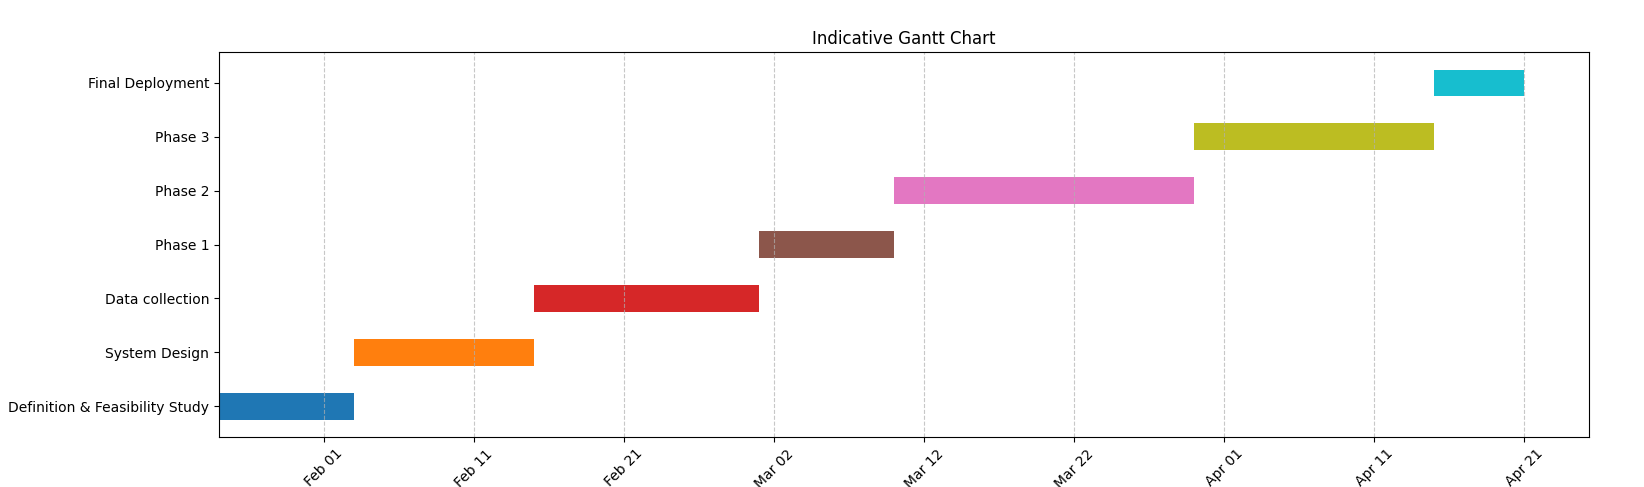
\includegraphics[width=0.8\textwidth]{gantt.png}
    \caption{Preliminary Planification Gantt Chart}
    \label{fig:gantt}
\end{figure}



\subsection{Glossary}
\begin{itemize}
    \item \textbf{AI (Artificial Intelligence)}: A system that simulates human intelligence to detect fraudulent behavior.
    \item \textbf{Proctoring}: The process of supervising an exam remotely to ensure integrity.
    \item \textbf{LMS (Learning Management System)}: A software application used to administer and deliver educational content.
\end{itemize}



\subsection{References}
For additional information, refer to the following resources:
\begin{itemize}
    \item ProctorU documentation: \url{https://www.proctoru.com/}
    \item Examity official site: \url{https://www.examity.com/}
    \item Proctorio features: \url{https://proctorio.com/}
\end{itemize}


\end{document}

